\documentclass[12pt,thmsa]{article}
\usepackage[french,english]{babel}
\usepackage[ansinew]{inputenc}
\usepackage[T1,OT1]{fontenc}
\usepackage{graphicx}
\usepackage{amsmath,amssymb,listings}
\usepackage{alltt,algorithmic,algorithm}
\usepackage{multicol}
\usepackage{multirow}
\usepackage{cite}
\usepackage{fancyhdr}
\usepackage{setspace}
\usepackage{array}
\usepackage{amsfonts}
\usepackage{latexsym}
\usepackage{epsf}
\usepackage{umlaute}
\usepackage{setspace}
\usepackage{amsthm}
\usepackage{enumerate}
\usepackage{stackrel}
\usepackage{amsmath}

\setlength{\textwidth}{160mm}
\setlength{\textheight}{230mm}
\setlength{\oddsidemargin}{-5mm}
\setlength{\topmargin}{-10mm}

% to get rid of the numbers in the bibliography:
\makeatletter
\def\@biblabel#1{}
\makeatother



\title{Assignement 5}




\begin{document}


\noindent \textsc{University of Geneva}     \hfill \textsc{Bachelor in Economics and Management} \\
\textbf{Probability 1}                      \hfill \textsc{Bachelor in International Relations} \\
Professor Davide La Vecchia                 \hfill Spring 2017  \\
ASSIGNMENT 05                               \hfill   March 27th



\noindent
\makebox[\linewidth]{\rule{\textwidth}{0.4pt}}\\[1.5ex]

\section*{Exercise 1}
You look at the following discrete probability distributions for two random variables X and Y respectively
\begin{center}
\begin{tabular}{l*{6}{c}r}
X \text{values}               & -1 & 1 & 3 & 5 & 7 \\
\hline
\text{Probability}         & 0.1 & 0.2 & 0.4 & 0.2 & 0.1  \\
\end{tabular}
\end{center}
\begin{center}
\begin{tabular}{l*{6}{c}r}
Y \text{values}               & -1 & 1 & 3 & 5 & 7 \\
\hline
\text{Probability}         & 0.2 & 0.15 & 0.3 & 0.15 & 0.2  \\
\end{tabular}
\end{center}

Compute the mean and the variance of both variables.\\


\noindent Solutions:\\
X and Y are discrete random variables. To calculate their expectations, we use \\ $ E(X)= \sum x\cdot P(X=x)$ \\
$ E(X)=(-1)\cdot 0.1+1\cdot 0.2+3\cdot 0.4+5\cdot 0.2+7\cdot 0.1=3 $\\
$ E(Y)=(-1)\cdot 0.2+1\cdot 0.15+3 \cdot 0.3+5\cdot 0.15+7 \cdot 0.2=3 $\\
$ E(X^{2})= \sum x^{2}\cdot P(X=x)=1^{2} \cdot 0.1+1^{2} \cdot 0.2+3^{2} \cdot 0.4+5^{2} \cdot 0.2+7^{2} \cdot 0.2=13.8 $\\
$ E(Y^{2})=\sum y^{2} \cdot P(Y=y)=1^{2} \cdot 0.2+1^{2} \cdot 0.15+3^{2} \cdot 0.3+5^{2} \cdot 0.15+7^{2} \cdot 0.2=16.6 $\\
Therefore the variance is \\
$ V(X)=E(X^{2})-E(X)^{2}=13.8-3^{2}=4.8 $\\
$ V(Y)=E(Y^{2})-E(Y)^{2}=16.6-3^{2}=7.6 $





\section*{Exercise 2}

In a TV game, a candidate faces 5 doors, one of which hides a gift. Viewers can make bets on the number of doors that the candidate will push until he finds the gift. Jules and Gaston are candidates for the game. Jules has a good memory and is not likely to push twice the same door. As far as Gaston is concerned, he has absolutely no memory.\\
\\
We denote the events as follows:
\begin{itemize}
\item $S$: `Success (there is a gift)';
\item $E$: `Failure (there is no gift)'.
\end{itemize}

\begin{enumerate}%[(a)]
\item Construct the probability function of the number of doors pushed by Jules. Calculate the expectation of this event.

Let $X$ be the random variable: Number of doors pushed by Jules. Jules remembers the doors he pushed. He will never push the same door twice:

\begin{center}
\begin{tabular}{|c|c|c|}
\hline
Event & $x_i$ & $P(X=x_i)$ \\[1mm]
\hline
\{S\} & 1 & $1/5$\\[1mm]
\hline
\{ES\} & 2 & $4/5\cdot 1/4=1/5$\\[1mm]
\hline
\{EES\} & 3 & $4/5\cdot 3/4\cdot 1/3=1/5$\\[1mm]
\hline
\{EEES\} & 4 & $4/5\cdot 3/4\cdot 2/3\cdot 1/2=1/5$\\[1mm]
\hline
\{EEEES\} & 5 & $4/5\cdot 3/4\cdot 2/3\cdot 1/2\cdot1=1/5$\\[1mm]
\hline
\end{tabular}
\end{center}

So
\begin{center}
$\mbox{E}(X) = \overset{5}{\underset{i=1}{\sum}}P(X=x_i)\cdot x_i = 1/5\cdot1+1/5\cdot2+1/5\cdot3+1/5\cdot4+1/5\cdot5=15/5=3. $
\end{center}

\item Construct the probability function of the number of doors pushed by Gaston. Calculate the expectation of this event.

\noindent \underline{Indication:} The following mathematical property can be used (generic geometric series):
$$|x|<1 \Rightarrow \sum_{k=1}^{\infty} k x^{k-1} = \frac{1}{(1-x)^2}.$$
Let $ Y $ be the random variable: Number of doors pushed by Gaston. Gaston does not remember the doors he pushed. It can be a bad door to infinity:
\begin{center}
\begin{tabular}{|c|c|c|}
\hline
Event & $y_i$ & $P(Y=y_i)$ \\[1mm]
\hline
\{S\} & 1 & $1/5$\\[1mm]
\hline
\{ES\} & 2 & $4/5\cdot 1/5=4/25$\\[1mm]
\hline
\{EES\} & 3 & $4/5\cdot 4/5\cdot 1/5=(4/5)^2\cdot(1/5)=16/125$\\[1mm]
\hline
\{EEES\} & 4 & $4/5\cdot 4/5\cdot 4/5\cdot 1/5=(4/5)^3\cdot(1/5)=64/625 $\\[1mm]
\hline
... & ... & ... \\[1mm]
\hline
\{$\underset{k-1}{\underbrace{EE..E}}S$\} & $k$ & $(4/5)^{k-1}\cdot(1/5)$\\[1mm]
\hline
\end{tabular}
\end{center}

So
\begin{center}
$\mbox{E}(Y) = \overset{\infty}{\underset{i=1}{\sum}}P(Y=y_i)\cdot y_i = \overset{\infty}{\underset{i=1}{\sum}}(1/5)\cdot(4/5)^{i-1}\cdot i=\frac{1/5}{(1-4/5)^2}=\frac{(1/5)}{(1/5)^2}=5. $\hspace{0.05cm} \footnote{Here, we use the property $\overset{\infty}{\underset{i=1}{\sum}}x^{i-1}\cdot i=\frac{1}{(1-x)^2}$.}
\end{center}

\item Generalize the previous results to n doors.
\begin{enumerate}%[(i)]
\item For Jules:

\begin{center}
\begin{tabular}{|c|c|c|}
\hline
Event & $x_i$ & $P(X=x_i)$ \\[1mm]
\hline
\{S\} & 1 & $1/n$\\[1mm]
\hline
\{ES\} & 2 & $(n-1)/n\cdot 1/(n-1)=1/n$\\[1mm]
\hline
\{EES\} & 3 & $(n-1)/n\cdot (n-2)/(n-1)\cdot 1/(n-2)=1/n$\\[1mm]
\hline
\{EEES\} & 4 & $(n-1)/n\cdot (n-2)/(n-1)\cdot (n-3)/(n-2)\cdot1/(n-3)=1/n $\\[1mm]
\hline
... & ... & ... \\[1mm]
\hline
\{$\underset{n-1}{\underbrace{EE..E}}S$\} & $n$ & $1/n$\\[1mm]
\hline
\end{tabular}
\end{center}

So
\begin{center}
$\mbox{E}(X) = \overset{n}{\underset{i=1}{\sum}}P(X=x_i)\cdot x_i = \frac{1}{n} \cdot(1+2+3+...+n)=\frac{\overset{n}{\underset{i=1}{\sum}}i}{n}=\frac{\frac{n\cdot(n+1)}{2}}{n}=\frac{n+1}{2}.$
\end{center}

\medskip

\item For Gaston:

\begin{center}
\begin{tabular}{|c|c|c|}
\hline
Event & $y_i$ & $P(Y=y_i)$ \\[1mm]
\hline
\{S\} & 1 & $1/n$\\[1mm]
\hline
\{ES\} & 2 & $((n-1)/n)\cdot (1/n)$\\[1mm]
\hline
\{EES\} & 3 & $((n-1)/n)^2\cdot (1/n)$\\[1mm]
\hline
\{EEES\} & 4 & $((n-1)/n)^3\cdot (1/n) $\\[1mm]
\hline
... & ... & ... \\[1mm]
\hline
\{$\underset{k-1}{\underbrace{EE..E}}S$\} & $k$ & $((n-1)/n)^{k-1}\cdot(1/n)$\\[1mm]
\hline
\end{tabular}
\end{center}

So
\begin{center}
$\mbox{E}(X) = \overset{\infty}{\underset{i=1}{\sum}}P(Y=y_i)\cdot y_i = \frac{1}{n}\cdot \overset{\infty}{\underset{i=1}{\sum}}(\frac{n-1}{n})^{i-1}\cdot i=\frac{1}{n}\cdot \frac{1}{(1-\frac{n-1}{n})^2}=\frac{1}{n}\cdot \frac{1}{(1/n)^2}=n.$
\end{center}

\end{enumerate}
\end{enumerate}


\section*{Exercise 3} %\bf Exercice 4.7 du recueil d'exercices}

Two cards are randomly chosen from a box containing the following five cards: 1, 1, 2, 2, 3. $X$ represents the average and $Y$ is the maximum of the two numbers drawn.
\begin{enumerate}%[(a)]
    \item Calculate the probability distribution, the cumulative distribution function, the mean and the variance of $X$, $Y$ and $Z = Y - X$. 

\medskip

It is assumed a draw without replacement.\\
  The total number of possible events is: $\binom{5}{2}=10$.
	\begin{center}
         	\begin{tabular}{|c|c|c|c|c|c|}
					\hline
 				 	Possible combinations & (1,1) & (1,2) & (1,3) & (2,2) & (2,3)\\[1mm]
					\hline
						Number of events & $\binom{2}{2}=1$ & $\binom{2}{1}\binom{2}{1}=4$ & $\binom{2}{1}\binom{1}{1}=2$ &  $\binom{2}{2} =1$ & 			 	          $\binom{2}{1}\binom{1}{1}=2$\\[1mm]
					\hline
												$x$ & 1 & 1.5 & 2 & 2 & 2.5\\[1mm]
					\hline
												$y$ & 1 & 2 & 3 & 2 & 3\\[1mm]
					\hline
												$z$ & 0 & 0.5 & 1 & 0 & 0.5\\[1mm]
					\hline
					
					\end{tabular}
         	\end{center}

The probability distribution, the distribution function, the mean and the variance can be calculated:

\begin{itemize}

\item 		For Variable $X$:
			
			\begin{center}
			\begin{tabular}{|c|c|c|c|c|}
			\hline
			$x$ & 1 & 1.5 & 2 & 2.5\\
			\hline
			$P(X=x)$ & 1/10 & 4/10 & 3/10 & 2/10\\
			\hline
			\end{tabular}
			\end{center}

			\medskip
			\begin{center}
			$F(x)=\begin{cases}
			0 & \begin{array}{cc} \textrm{if} & x<1\end{array}\\
			1/10 & \begin{array}{cc} \textrm{if} & 1\leq x<1.5\end{array}\\
			5/10 & \begin{array}{cc} \textrm{if} & 1.5\leq x<2\end{array}\\
			8/10 & \begin{array}{cc} \textrm{if} & 2\leq x<2.5\end{array}\\
			1 & \begin{array}{cc} \textrm{if} & x\geq2.5\end{array}
			\end{cases}$
			\end{center}

\begin{center}
			$\mbox{E}(X) = \overset{4}{\underset{i=1}{\sum}}P(X=x_i)\cdot x_i = 1/10\cdot1 + 4/10\cdot1.5 + 				3/10\cdot2 + 2/10\cdot2.5 = 1.8$ \\
			$\mbox{E}(X^2) = \overset{4}{\underset{i=1}{\sum}}P(X=x_i)\cdot x_i^2 = 1/10\cdot1^2 + 						4/10\cdot1.5^2 + 3/10\cdot2^2 + 2/10\cdot2.5^2 = 3.45 $\\
			$\mbox{var}(X) =  \mbox{E}(X^2) - \mbox{E}(X)^2 = 3.45 - 1.8^2 = 0.21$
\end{center}

\item 		For Variable $Y$:
			\begin{center}
			\begin{tabular}{|c|c|c|c|}
			\hline
			$y$ & 1 & 2 & 3 \\
			\hline
			$P(Y=y)$ & 1/10 & 5/10 & 4/10\\
			\hline
			\end{tabular}
			\end{center}

			\medskip
			\begin{center}
			$F(y)=\begin{cases}
			0 & \begin{array}{cc} \textrm{if} & y<1\end{array}\\
			1/10 & \begin{array}{cc} \textrm{if} & 1\leq y<2\end{array}\\
			6/10 & \begin{array}{cc} \textrm{if} & 2\leq y<3\end{array}\\
			1 & \begin{array}{cc} \textrm{if} &  y\geq 3\end{array}
			\end{cases}$
			\end{center}

			\begin{center}
			$\mbox{E}(Y) = \overset{3}{\underset{i=1}{\sum}}P(Y=y_i)\cdot y_i = 1/10\cdot1 + 5/10\cdot 2 + 4/10\cdot3 = 2.3$ \\
			$\mbox{E}(Y^2) = \overset{3}{\underset{i=1}{\sum}}P(Y=y_i)\cdot y_i^2 = 1/10\cdot1^2 + 5/10\cdot 2^2 + 4/10\cdot3^2 = 5.7 $\\
			$\mbox{var}(Y) =  \mbox{E}(Y^2) - \mbox{E}(Y)^2 = 5.7 - 2.3^3 = 0.41$
			\end{center}
			\bigskip

\item 		For Variable $Z$:
			\begin{center}
			\begin{tabular}{|c|c|c|c|}
			\hline
			$z$ & 0 & 0.5 & 1 \\
			\hline
			$P(Z=z)$ & 2/10 & 6/10 & 2/10\\
			\hline
			\end{tabular}
			\end{center}

			\medskip
			\begin{center}
			$F(z)=\begin{cases}
			0 & \begin{array}{cc} \textrm{if} & z<0\end{array}\\
			2/10 & \begin{array}{cc} \textrm{if} & 0\leq z<0.5\end{array}\\
			8/10 & \begin{array}{cc}	\textrm{if} & 0.5\leq z<1\end{array}\\
			1 & \begin{array}{cc} \textrm{if} &  z\geq 1\end{array}
			\end{cases}$
			\end{center}

			\begin{center}
			$\mbox{E}(Z) = \overset{3}{\underset{i=1}{\sum}}P(Z=z_i)\cdot z_i = 2/10\cdot0 + 6/10\cdot0.5 + 2/10\cdot1 = 0.5$ \\
			$\mbox{E}(Z^2) = \overset{3}{\underset{i=1}{\sum}}P(Z=z_i)\cdot z_i^2 = 2/10\cdot0^2 + 6/10\cdot0.5^2 + 2/10\cdot1^2 = 0.35 $\\
			$\mbox{var}(Z) =  \mbox{E}(Z^2) - \mbox{E}(Z)^2 = 0.35 - 0.5^2 = 0.1$		
			\end{center}

\end{itemize}		
    \item If $W$ is the sum of the two numbers, what are its expectation and its variance?

We can calculate the values of $ W $ for each possible case, and draw the table as we did for the variables $ X $, $ Y $ and $ Z $ to obtain the probability function then the mean and the variance of $ W $. However, it is faster to note that:
\begin{center}
$\displaystyle X= \frac{\textrm{Card 1} + \textrm{Card 2}}{2}=\frac{\textrm{Sum of the numbers of the two cards}}{2}.$
\end{center}
So we have:
\begin{center}

$W$ = Sum of the numbers of the two cards = $2X$
\medskip

$\mbox{E}(W) = \mbox{E}(2X) = 2\mbox{E}(X) = 2 \cdot 1.8 = 3.6$
\medskip

$\mbox{var}(W) = \mbox{var}(2X) = 2^2\mbox{var}(X) = 4\cdot 0.21 = 0.84$

\end{center}

\end{enumerate}




\section*{Exercise 4} %\bf}

We consider a die whose faces are numbered from 1 to 6 and we define $X$ the random variable given by the number of the upper face. It is assumed that the die is rigged so that the probability of getting a face is proportional to the number on that face.

 \begin{enumerate}%[(a)]
\item Determine the probability function of $X$, then calculate its expectation and variance.\\

By the proportionality assumption, we know that there exists $\alpha \in \mathbb{R}$ such that $P(X=k)=\alpha k$, $\forall k=1,\ldots,6$. Moreover, since the sum of the probabilities associated with the different faces must always be equal to 1, we have $\sum\limits_{k=1}^6 P(X=k)=1$. By combining these two equations, we obtain $\sum\limits_{k=1}^6 \alpha k=\alpha \sum\limits_{k=1}^6 k=21 \alpha=1 \iff \alpha=\frac{1}{21}$. We can therefore establish the probability function of $ X $ as follows:
			\begin{center}
			\begin{tabular}{|c|c|c|c|c|c|c|}
			\hline
			$x$ & 1 & 2 & 3 & 4 & 5 & 6 \\
			\hline
			$P(X=x)$ & 1/21 & 2/21 & 3/21 & 4/21 & 5/21 & 6/21\\
			\hline
			\end{tabular}
			\end{center}

We can then calculate the expectation as follows:

\begin{center}
$\mbox{E}(X) = \overset{6}{\underset{x=1}{\sum}}P(X=x)\cdot x = 1/21\cdot1 + 2/21\cdot 2 + 3/21\cdot3+4/21 \cdot 4 +5/21 \cdot 5+6/21 \cdot 6 =13/3.$
\end{center}

As for the variance, we have:
\begin{equation*}
\begin{split}
\mbox{var}(X) & = \overset{6}{\underset{x=1}{\sum}}P(X=x)\cdot x^2 -\mbox{E}(X)^2 \\
& = 1/21\cdot1^2 + 2/21\cdot 2^2 + 3/21\cdot3^2+4/21 \cdot 4^2 +5/21 \cdot 5^2+6/21 \cdot 6^2 -(13/3)^2 \\
& =20/9.
\end{split}
\end{equation*}

\item We define $Y = 3X$. Calculate the expectation and variance of $Y$. Is it necessary to determine the probability function of $Y$ for calculating its expectation and variance?\\

The expectation and variance of $ Y $ can be calculated without determining its probability function. Indeed, since $Y=3X$, we have $\mbox{E}(Y)=\mbox{E}(3X)=3\mbox{E}(X)=3\cdot 13/3=13$ and $\mbox{var}(Y)=\mbox{var}(3X)=3^2\mbox{var}(X)=9\cdot 20/9=20$.

\item We define $Z = \frac{1}{X}$. Calculate the expectation and variance of $Z$. Is it necessary to determine the probability function of $Z$ for calculating its expectation and variance?\\

Here it is necessary to determine the probability function of $ Z $. In general $\mbox{E}(1/X) \neq 1/\mbox{E}(X)$. Given that $z=1/x, \quad \forall x=1,\ldots,6$, the probability function of $ Z $ is easily obtained:

			\begin{center}
			\begin{tabular}{|c|c|c|c|c|c|c|}
			\hline
			$z$ & 1 & 1/2 & 1/3 & 1/4 & 1/5 & 1/6 \\
			\hline
			$P(Z=z)$ & 1/21 & 2/21 & 3/21 & 4/21 & 5/21 & 6/21\\
			\hline
			\end{tabular}
			\end{center}

Then we can calculate the expectation and the variance of $ Z $:
\begin{equation*}
\begin{split}
\mbox{E}(Z) & = \overset{6}{\underset{k=1}{\sum}}P(Z=1/k)\cdot 1/k \\
& = 1/21\cdot1 + 2/21\cdot 1/2 + 3/21\cdot 1/3+4/21 \cdot 1/4 +5/21 \cdot 1/5+6/21 \cdot 1/6 \\&= 6/21 =2/7
\end{split}
\end{equation*}

\begin{equation*}
\begin{split}
\mbox{var}(Z) & = \overset{6}{\underset{k=1}{\sum}}P(Z=1/k)\cdot (1/k)^2 -\mbox{E}(Z)^2  \\
& = 1/21\cdot 1^2 + 2/21\cdot (1/2)^2 + 3/21\cdot (1/3)^2+4/21 \cdot (1/4)^2 +5/21 \cdot (1/5)^2\\&+6/21 \cdot (1/6)^2 -(2/7)^2  = 103/2940
\end{split}
\end{equation*}
\end{enumerate}


\section*{Exercise 5} %\bf}

\begin{enumerate}
\item The following game is considered: The player rolls a fair six sided die once. If he gets 1, 2 or 3, he wins the equivalent in francs. Otherwise, he loses 2 francs. Let $ X $ be the random variable corresponding to the player's win (a negative value indicating a loss).

\begin{enumerate}%[(a)]
\item Give the probability function of $X$ and its distribution function $F_X$.\\

Since the die is not rigged, each face has the same probability of occurrence, {\it i.e.} $ 1/6 $. The probability function of $ X $ is therefore the following:

			\begin{center}
			\begin{tabular}{|c|c|c|c|c|}
			\hline
			$x$ & -2 & 1 & 2 & 3 \\
			\hline
			$P(X=x)$ & 1/2 & 1/6 & 1/6 & 1/6\\
			\hline
			\end{tabular}
			\end{center}

The distribution function, $ F_X $, is written as follows:

            \begin{center}
			$F_X(x)=\begin{cases}
			0 & \begin{array}{cc} \textrm{if} & x<-2\end{array}\\
			1/2 & \begin{array}{cc} \textrm{if} & -2\leq x<1\end{array}\\
			2/3 & \begin{array}{cc}	\textrm{if} & 1\leq x<2\end{array}\\
            5/6 & \begin{array}{cc}	\textrm{if} & 2\leq x<3\end{array}\\
			1 & \begin{array}{cc} \textrm{if} &  x\geq 3\end{array}
			\end{cases}$
			\end{center}

\item Calculate the expectation and variance of $X$.\\

Using the probability function of $ X $, we can easily calculate the expectation and the variance:

\begin{center}
$\mbox{E}(X) = 1/2\cdot (-2) + 1/6 \cdot 1 + 1/6 \cdot 2+1/6 \cdot 3=0$; \\
$\mbox{var}(X) =  1/2\cdot (-2)^2 + 1/6 \cdot 1^2 + 1/6 \cdot 2^2+1/6 \cdot 3^2-0^2=13/3.$
\end{center}
\end{enumerate}

\item We modify the game as follows: The winnings remain the same for the results 1, 2 or 3, but if the player gets something else, he rolls the die again. If he then gets 3 or less, he wins 3 francs, otherwise he loses 5 francs. We define $Y$ as the random variable corresponding to the gain of the player in this new game.

\begin{enumerate}%[(a)]
\item Give the probability function of $Y$ and its distribution function $F_Y$.\\

We can start by considering the outcomes where the game stops after the first roll of the die. There are three possibilities, each having a probability of $1/6$, and the values of $ Y $ associated with these three outcomes are 1, 2, and 3. If the player must raise the die again (which happens with a probability of $ 1/2$), then there are two possibilities, each having a conditional probability (of having to roll the die at the second time) of $ 1/2$, and the values of $ Y $ are then 3 and -5 . It can be useful to represent this game by means of a probability tree:

\begin{center}
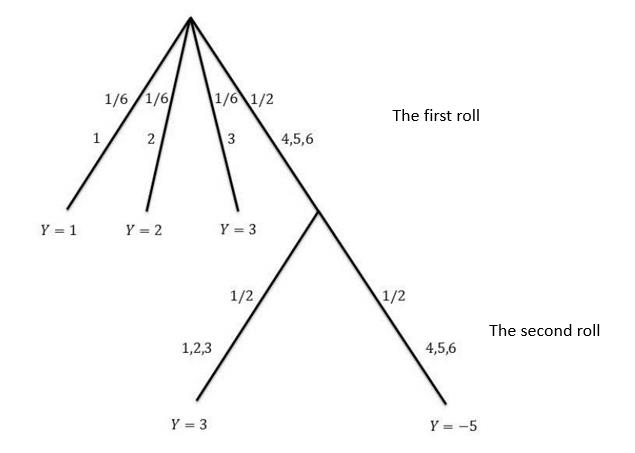
\includegraphics[scale=0.8]{Arbre_1.jpg}
\end{center}

Therefore, the probability function of $Y$ is \footnote{$P(Y=3)=1/6+1/2 \cdot 1/2=5/12$.}:

			\begin{center}
			\begin{tabular}{|c|c|c|c|c|}
			\hline
			$y$ & -5 & 1 & 2 & 3 \\
			\hline
			$P(Y=y)$ & 1/4 & 1/6 & 1/6 & 5/12 \\
			\hline
			\end{tabular}
			\end{center}

The distribution function, $ F_Y $, is the following:

            \begin{center}
			$F_Y(y)=\begin{cases}
			0 & \begin{array}{cc} \textrm{if} & y<-5\end{array}\\
			1/4 & \begin{array}{cc} \textrm{if} & -5\leq y<1\end{array}\\
			5/12 & \begin{array}{cc}	\textrm{if} & 1\leq y<2\end{array}\\
            7/12 & \begin{array}{cc}	\textrm{if} & 2\leq y<3\end{array}\\
			1 & \begin{array}{cc} \textrm{if} &  y\geq 3\end{array}
			\end{cases}$
			\end{center}
\item Calculate the expectation and variance of $Y$.\\

Using the probability function of $Y$, expectancy and variance are easily calculated:

\begin{center}
$\mbox{E}(Y) = 1/4\cdot (-5) + 1/6 \cdot 1 + 1/6 \cdot 2+5/12 \cdot 3=1/2$; \\
$\mbox{var}(Y) =   1/4\cdot (-5)^2 + 1/6 \cdot 1^2 + 1/6 \cdot 2^2+5/12 \cdot 3^2-(1/2)^2=127/12$.
\end{center}
\end{enumerate}

\item Which game is the most advantageous for the player? To justify.\\

It depends on the player's preferences. Indeed, we notice that $ 0 = \mbox {E} (X) <\mbox {E} (Y) $, which would seem to indicate that the second variable is preferable because, on average, the player should earn money with this but not with the first variable. However, we also have $ \mbox {var} (X) <\mbox {var} (Y) $, sign of a greater variability of the gain with the second variable. The maximum potential loss in this second variable of the game is also much larger (in relative terms). If the player desires to avoid it at all costs, he may prefer the first game despite a lower expectation of gain.

\end{enumerate}


\section*{Exercise 6 (Optional)}
The random variable $ X $ is Bernoulli(p) distribution if its probability mass function is given by:
\begin{align*}
P(X=x)=p^{x}(1-p)^{1-x} & \text{for } x=0,1
\end{align*}
where $ 0<p<1 $.
Compute the Mean and the Variance of the Bernoulli distribution.\\

\noindent Solutions:\\
\noindent $ E(X)= \sum x\cdot P(X=x)=1\cdot p+0\cdot (1-p)=p $\\
$ E(X^{2})=\sum x^{2}\cdot P(X=x)=1^{2}\cdot p+0^{2}\cdot (1-p)=p $\\
Therefore the variance is \\
$ V(X)=E(X^{2})-E(X)^{2}=p-p^{2}=p(1-p) $\\






\section*{Exercise 7 (Optional)}

Let $X$ a discrete random variable following a Poisson distribution with parameter $\lambda$. Its probability function is given by:
\begin{equation*}
P(X=k)=e^{-\lambda} \frac{\lambda^{k}}{k!} \quad \text{for} \quad k=0,1,...
\end{equation*}
\begin{enumerate}
  \item Check that $P(X=k)$ is a probability function.
  \item Proove that its expectation is equal to $\lambda$.
  \item Find the variance of $X$.
  \item Compare the expectation and the variance of $X$ with the expectation and the variance of $S$ found in Exercise 4 above, for a very large $n$.
\end{enumerate}

\noindent Solutions:
\begin{enumerate}
  \item We have to check that the probability function is positive and that it sums up to 1.
  \begin{equation*}
  \sum_{k=0}^{\infty} e^{-\lambda} \frac{\lambda^{k}}{k!}=e^{-\lambda} \sum_{k=0}^{\infty} \frac{\lambda^{k}}{k!}=e^{-\lambda} e^{\lambda}=1
  \end{equation*}
  \item \begin{eqnarray*}
    E(X) &=& \sum_{k=0}^{\infty} k e^{-\lambda} \frac{\lambda^{k}}{k!} = \lambda \sum_{k=1}^{\infty}  e^{-\lambda}  \frac{\lambda^{k-1}}{(k-1)!} \\
    &=& \lambda \sum_{j=0}^{\infty}  e^{-\lambda}  \frac{\lambda^{j}}{(j)!} = \lambda  \quad \text{for } j=k-1
  \end{eqnarray*}

 \item  \begin{eqnarray*}
E(X^2) &=& \sum_{k=0}^{\infty} k^2 e^{-\lambda} \frac{\lambda^{k}}{k!} = \lambda \sum_{k=1}^{\infty} k e^{-\lambda} \frac{\lambda^{k}}{(k-1)!} \\ 
& \overset{\text{j=k-1}}{=} & \sum_{j=0}^{\infty} (j+1) e^{-\lambda}  \frac{\lambda^{j+1}}{(j)!} \\
&=& \lambda \{ \underbrace{\sum_{j=0}^{\infty} j e^{-\lambda}  \frac{\lambda^{j}}{(j)!}}_{E(X)=\lambda} + \sum_{j=0}^{\infty}  e^{-\lambda}  \frac{\lambda^{j}}{(j)!}\} \\
&=& \lambda (\lambda+1)
\end{eqnarray*}

  $ V(X) = E(X^2) - E(X)^2 = \lambda ( \lambda +1) - \lambda ^2 =\lambda $\\

\item Let us denote the expected value of the binomial distribution, np by $ \lambda $, which means $ p=\frac{n}{\lambda} $.  Now, if we use this to rewrite P(S=x) in terms of $\lambda$, n, and x, we obtain \\
\begin{eqnarray*}
P(S = x) &= & \left( { n \atop x } \right)(\frac{n}{\lambda})^x(1-{\frac{n}{\lambda}})^{n-x}  = \frac{n(n-1) \cdots (n-x+1)}{(x)!}\frac{\lambda^x}{n^x}(1-\frac{\lambda}{n})^{n-x}\\ 
& = & \frac{n}{n}\times \frac{n-1}{n} \cdots \frac{n-x+1}{n} \times \frac{\lambda^x}{(x)!}(1-\frac{\lambda}{n})^{n-x}\\
&=& \frac{n}{n}\times \frac{n-1}{n} \cdots \frac{n-x+1}{n} \times \frac{\lambda^x}{(x)!}(1-\frac{\lambda}{n})^{n}(1-\frac{\lambda}{n})^{-x}\\ 
\end{eqnarray*}
If we tool the limit as n approaches infinity, keeping x and $\lambda$ fixed,the first x fractions in this expression would tend towards 1, as would the last factor in the expression. $ \lim_{x\to\infty} (1-\frac{\lambda}{n})^{n} =  e^{-\lambda}, so \lim_{x\to\infty}P(S=x)= \frac{e^{-\lambda}{\lambda}^x}{x!} $\\
So we can say expectations and variances of X and S are equivalent for a very large n. The Poisson distribution is actually a limiting case of a Binomial distribution when the number of trials, n, gets very large and p, the probability of success, is small.

 
\end{enumerate}




\end{document}



